Before delving into methodologies, we explain terms used in the paper.
\textbf{Notes}: In Figure~\ref{fig:stepmania}, we see arrows that travel upwards.
These arrows, are known as notes, think musical notes.

\textbf{Receptor}: They all travel towards the \textbf{Receptor}, the grayed out arrows, where the player must press the respective keys when the notes line up with the receptors.

\textbf{Long Notes (LN)}: There are 2 types of notes in Figure~\ref{fig:stepmania}, one an arrow, the other an arrow with a long blue tail.
The note with a tail means the player must press down for the whole duration of the body.

\textbf{Keys}: Observe Figure~\ref{fig:stepmania}'s 4 columns, this implies the number of keys is 4.
Some games such as:
\begin{itemize}
    \item~\cite{quaver} has 4 and 7 Keys
    \item~\cite{osu} has 1 to 18 Keys
    \item~\cite{etterna} has only 4 Keys
    \item~\cite{o2jam} has 7 Keys
\end{itemize}

By popular convention, $n$ Keys are shortened to $n$K; 4 Keys are usually called 4K.

\subsection{Standard ASCII Format}\label{subsec:standard-ascii-format}

For the rest of the paper, to make it simple, we use a easy to understand representation in ASCII.

Observe the following conversion of Figure~\ref{fig:stepmania}'s left play field

\begin{figure}[H]
    \centering
    \begin{minipage}{.5\textwidth}
        \centering
        \begin{centeredverbatim}
            | Receptor |
            | ======== |
            |       >  |
            | <        |
            |     ^    |
            |          |
            | <   ^    |
            | |        |
            | |        |
        \end{centeredverbatim}
    \end{minipage}%
    \begin{minipage}{0.5\textwidth}
        \centering
        \begin{centeredverbatim}
            | |        |
            | |        |
            | O O      |
            |          |
            |          |
            |     O    |
            | O        |
            |       O  |
            | ======== |
            | Receptor |
        \end{centeredverbatim}
    \end{minipage}
    \caption{Figure~\ref{fig:stepmania} Left Stage in ASCII. Left: Before Standardization, Right: Standardized Format.}
    \label{fig:fig3ascii}
\end{figure}

We simplify all to \verb+O+ and make them scroll downwards \footnote{This is commonly known as down-scroll.} in Figure~\ref{fig:fig3ascii}.
Observe that they are the same pattern, just vertically flipped.

We illustrate a few more examples for your digestion.

\begin{figure}[H]
    \centering
    \begin{minipage}{.5\textwidth}
        \centering
        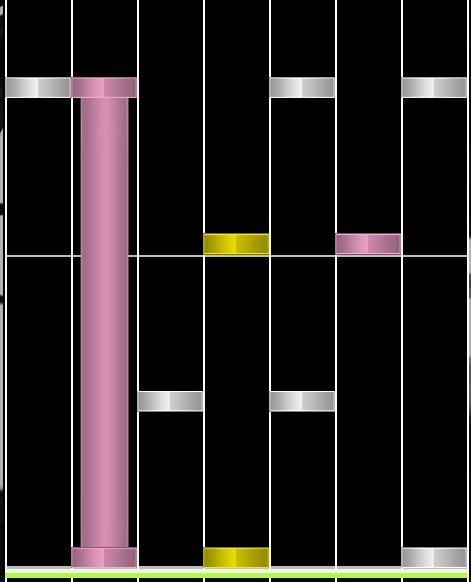
\includegraphics[scale=0.3]{imgs/osupattern}
    \end{minipage}%
    \begin{minipage}{0.5\textwidth}
        \centering
        \begin{verbatim}
O |     O   O
  |   O   O
  | O   O
  O   O     O
=============
        \end{verbatim}
    \end{minipage}
    \caption{7K Pattern in osu! editor}
    \label{fig:osupattern}
\end{figure}

\begin{figure}[H]
    \centering
    \begin{minipage}{.5\textwidth}
        \centering
        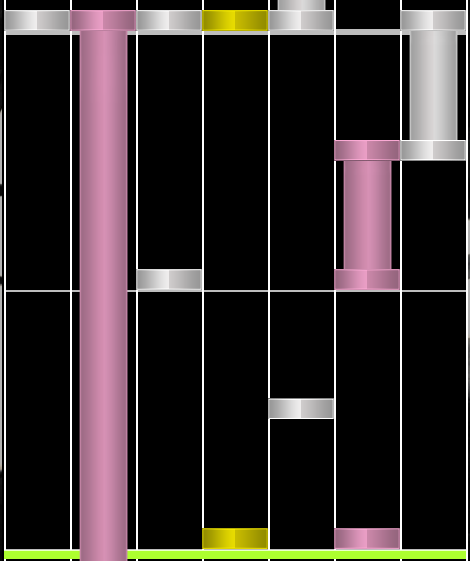
\includegraphics[scale=0.3]{imgs/osupattern2}
    \end{minipage}%
    \begin{minipage}{0.5\textwidth}
        \centering
        \begin{verbatim}
O | O O O   |
  |       | O
  | O     O
  |     O
  |   O   O
=============
        \end{verbatim}
    \end{minipage}
    \caption{7K Pattern in osu! editor (2)}
    \label{fig:osupattern2}
\end{figure}

\begin{figure}[H]
    \centering
    \begin{minipage}{.5\textwidth}
        \centering
        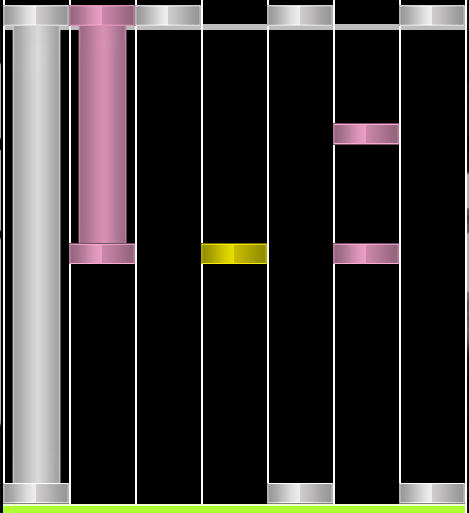
\includegraphics[scale=0.3]{imgs/osupattern3}
    \end{minipage}%
    \begin{minipage}{0.5\textwidth}
        \centering
        \begin{verbatim}
| | O   O   O
| |       O
| O   O   O
|
|       O   O
=============
        \end{verbatim}
    \end{minipage}
    \caption{7K Pattern in osu! editor (3)}
    \label{fig:osupattern3}
\end{figure}

